\documentclass[10pt,a4paper]{article}
\usepackage[paper=a4paper, hmargin=1.5cm, bottom=1.5cm, top=3.5cm]{geometry}

\usepackage[utf8]{inputenc}
\usepackage[spanish]{babel}

\usepackage{mathtools}
\usepackage{amsmath}
\usepackage{amsfonts}
\usepackage{amssymb}
\usepackage{listings}


\usepackage{booktabs}
\usepackage[table,xcdraw]{xcolor} % for setting colors
\usepackage{ifthen}
\usepackage{enumitem}
\usepackage{setspace}
\usepackage{wrapfig}

\usepackage{graphicx}
\usepackage{epstopdf}
\usepackage{tikz}
\usepackage[framemethod=tikz]{mdframed}

\usepackage{listings}
\usepackage{algpseudocode}

\DeclarePairedDelimiter{\ceil}{\lceil}{\rceil}

% set the default code style
\lstset{
    frame=tb, % draw a frame at the top and bottom of the code block
    tabsize=4, % tab space width
    showstringspaces=false, % don't mark spaces in strings
    %numbers=left, % display line numbers on the left
    commentstyle=\color{green}, % comment color
    keywordstyle=\color{blue}, % keyword color
    stringstyle=\color{red} % string color
}

\title{Organización del Computador II \\ TP2}

\newcommand{\order}[1]{$\mathcal{O}(#1)$}

%%%%%%%%%% Macros misceláneos - Inicio %%%%%%%%%%
\newcommand{\xmm}[1]{\texttt{XMM#1}\ }
\newcommand{\rax}{\texttt{RAX}\ }
\newcommand{\rbx}{\texttt{RBX}\ }
\newcommand{\rcx}{\texttt{RCX}\ }
\newcommand{\rdx}{\texttt{RDX}\ }
\newcommand{\rbp}{\texttt{RBP}\ }
\newcommand{\rsp}{\texttt{RSP}\ }
\newcommand{\mem}{\texttt{MEM}\ }
\newcommand{\reg}[1]{\texttt{R#1}\ }
\newcommand{\asm}[1]{\texttt{\uppercase{#1}}\ }
%%%%%%%%%% Macros misceláneos - Fin %%%%%%%%%%

% Registros
\newcommand{\regfloats}[4]{\begin{tabular}{|c|c|c|c|}\hline
  #1 & #2 & #3 & #4 \\ \hline \end{tabular}}

\newcommand{\regintOcho}[8]{\begin{tabular}{|c|c|c|c|c|c|c|c|}\hline
  #1 & #2 & #3 & #4 & #5 & #6 & #7 & #8  \\ \hline \end{tabular}}

\onehalfspacing
\begin{document}

%% cover page

\maketitle

\bigskip

\begin{table}[h]
\centering
\begin{tabular}{|l l l|}
\hline
Integrante       & \multicolumn{1}{c}{LU}     & Correo electrónico        \\ \hline
Martin Baigorria & \multicolumn{1}{c}{575/14} & martinbaigorria@gmail.com \\ 
Martin Baigorria & 575/14                      & martinbaigorria@gmail.com \\
Gonzalo Ciruelos Rodríguez & 063/14           & gonzalo.ciruelos@gmail.com \\ \hline
\end{tabular}
\end{table}

\vfill

\begin{center}
\textbf{Reservado para la cátedra}
\end{center}
\begin{table}[h]
\centering
\begin{tabular}{|l|l|l|}
\hline
Instancia       & Docente & Nota \\ \hline
Primera entrega &         &      \\ \hline
Segunda entrega &         &      \\ \hline
\end{tabular}
\end{table}


\tableofcontents

% end cover page

\pagebreak

\section{Introducción}

El presente trabajo practico tiene como objetivo aprender a utilizar instrucciones que operan con múltiples datos SIMD (Single instruction, multiple data), soportada por la familia de procesadores x86-64 de Intel. En general, este tipo de instrucciones se utilizan mucho en procesamiento digital de señales y procesamiento de gráficos. Debido a restricciones de la cátedra, solo utilizaremos SSE (Streaming SIMD Extensions) y no el set de instrucciones mas nuevo AVX (Advanced Vector Extensions).
 
\subsection{Historia}
 
\begin{wrapfigure}{r}{0.3\textwidth}
  \begin{center}
    
\includegraphics[scale=0.2]{pentium.jpg}
  \end{center}
  \caption{Intel Pentium P5}
  \begin{center}
    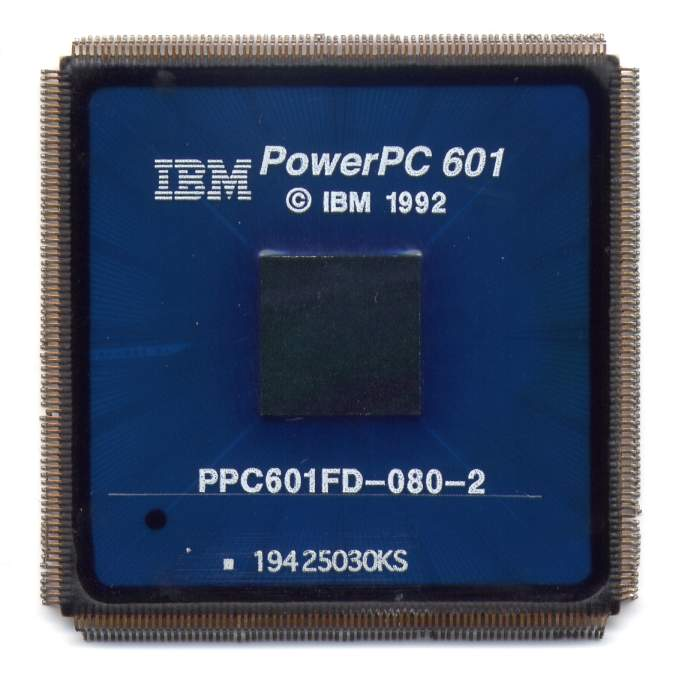
\includegraphics[scale=1.5]{powerpc.jpg}
  \end{center}
  \caption{Power PC}
\end{wrapfigure} 
 
El set de instrucciones MMX (MultiMedia eXtension) fue el primero en implementar SIMD en la arquitectura Intel en el año 1997, con los procesadores Pentium II. La idea era, como lo indica el nombre, permitir el procesamiento de operaciones sobre múltiples datos en simultaneo. Esto en general se conoce como paralelismo a nivel de datos, donde un único proceso es capaz de ejecutar estas instrucciones.

MMX define 8 nuevos registros de 64 bits, desde el MM0 al MM7. A nivel arquitectura, estos registros eran simplemente un alias de los registros de la FPU, por lo que cualquier operación en la FPU afecta a los registros MM$i$.

En el año 1999, con el objetivo de responder a las mejoras introducidas por la competencia, en general por el AltiVec en las PowerPc de Motorola y el sistema POWER de IBM, Intel introduce el set de instrucciones SSE con la serie de procesadores Pentium III. El set de instrucciones SSE tenia 70 nuevas instrucciones. Aquí Intel agrega 8 nuevos registros de 128 bits, XMM0 a XMM7, independientes de la FPU. Este set de instrucciones luego se actualizo con SSE2 (2001), SSE3 (2004), SSSE3 (2006) y SSE4(2006).

En el año 2011 finalmente se introduce al mercado las extensiones al set de instrucciones AVX (Advanced Vector Extensions), primero implementado por la linea de procesadores de Intel Sandy Bridge. AVX expande el tamaño de los registros de 128 a 256 bits, y se renombra a estos registros como YMM0-YMM7. Introduce las operaciones vectorizadas de tres operandos. 

Intel introduce AVX2 en el año 2013 con la linea de procesadores Haswell, que expande muchas de las instrucciones de SSE y AVX a 256 bits.

Actualmente Intel esta por lanzar este año la linea de procesadores Xeon Phi Knights Landing, que busca expandir las operaciones y los registros de AVX2 a 512 bits.

\subsection{Filtros de Imágenes}

Una aplicación típica de este tipo de instrucciones es el procesamiento de imágenes. Esto se debe a que una imagen esta representada por un mapa de píxeles, y en general al procesar imágenes se esta llevando a cabo el mismo tipo de procedimiento muchas veces. A continuación se analizaremos algunos filtros de imágenes, técnicas de implementación de los mismos, y haremos un análisis cuantitativo de las diferencias entre ellos, así como posibles mejoras y reflexiones respecto de las implementaciones puntuales.

A fines de simplificar el análisis, solo utilizaremos imágenes de tamaño $HxW$ en formato bmp, tal que $w$ sea múltiplo de 4. Notaremos a $i$ como el índice de las filas, a $j$ como el índice de las columnas y a $k$ como el índice de los componentes de color de cada píxel. $m_{i, j, k}$ por lo tanto sera el componente $k$ del píxel asociado a la fila $i$, columna $j$.

\newpage

\section{Blur}

\subsection{Introducción}
Blur es un filtro que suaviza la imagen. Esto lo hace asignándole a cada píxel el promedio (media aritmética) con sus píxeles vecinos. Es decir:

$$m_{i, j} = (m_{i-1, j-1} + m_{i-1, j} + m_{i-1, j+1} + m_{i, j-1} + m_{i, j} + m_{i, j+1} + m_{i+1, j-1} + m_{i+1, j} + m_{i+1, j+1}) / 9$$

Las consecuencias de adoptar este método son fundamentalmente dos; en primer lugar, nótese que esto significa que no vamos a procesar los píxeles en los bordes, ya que no tienen la cantidad suficiente de píxeles vecinos.

En segundo lugar, debemos tener en cuenta que el cálculo de blur en particular requiere utilizar datos de los elementos anteriormente procesados. Esto significa que es imposible procesar la imagen con una complejidad espacial de \order{1}, dado que no podemos simplemente guardar nuestros resultados en la misma imagen. Evaluamos dos formas de solucionar este problema:

\begin{itemize}
\item La primera, crear una nueva matriz en memoria con las mismas dimensiones que la matriz procesada, para poder calcular utilizando los datos originales y guardar en esta matriz. Este método tiene la desventaja de tener una complejidad espacial de $O(w*h)$, fuera de que se agrega un $O(w*h)$ de complejidad temporal para copiar los datos desde la nueva matriz creada hacia la matriz original. Además, este método tiene la desventaja de tener que cuidarse en el copiado para no sobre escribir el borde de la matriz original.

\item La segunda, seguir la metodología utilizada en el código de C provisto por la cátedra: mantener dos punteros a memoria de tamaño $w$ que guarden las dos primeras filas originales de la matriz que estamos procesando, y vayan corriéndose a medida que aumentamos la cantidad de filas. Este método toma $O(w)$ de complejidad espacial, con un $O(w)$ de complejidad temporal en el ciclo principal de las filas, para poder copiar los nuevos datos. La ventaja de este método con respecto al anterior reside en el menor uso de memoria, ya que en términos de complejidad temporal el trabajo se amortiza a lo largo de los ciclos.
\end{itemize}

Terminamos optando por el segundo método, en favor de la mejoría de complejidad espacial a cambio de un golpe en la dificultad conceptual del algoritmo y su código fuente. Procedemos a desarrollar los casos particulares de nuestras implementaciones.

\subsection{ASM1}

Siguiendo la idea del código en C, ASM1 recorre el mapa de píxeles de la misma manera. El código en C procesa cada componente del píxel por separado, mientras que la idea de esta versión es procesar todos los componentes de un píxel con SSE. La idea nuevamente es iterar toda la imagen, primero por filas y luego por columnas, reemplazando los píxeles en las posiciones correspondientes.

\begin{table}[h]
\centering
\mem
\begin{tabular}{l|c|c|c|c|l}
 & \multicolumn{1}{l|}{}      & \multicolumn{1}{l|}{}       & \multicolumn{1}{l|}{}       & \multicolumn{1}{l|}{}       &  \\ \hline
 & \cellcolor[HTML]{FFCB2F}P1 & \cellcolor[HTML]{FFCB2F}P2  & \cellcolor[HTML]{FFCB2F}P3  & \cellcolor[HTML]{FD6864}P4  &  \\ \hline
 & \cellcolor[HTML]{FFCB2F}P5 & \cellcolor[HTML]{FFFC9E}P6  & \cellcolor[HTML]{FFCB2F}P7  & \cellcolor[HTML]{FD6864}P8  &  \\ \hline
 & \cellcolor[HTML]{FFCB2F}P9 & \cellcolor[HTML]{FFCB2F}P10 & \cellcolor[HTML]{FFCB2F}P11 & \cellcolor[HTML]{FD6864}P12 &  \\ \hline
 & \multicolumn{1}{l|}{}      & \multicolumn{1}{l|}{}       & \multicolumn{1}{l|}{}       & \multicolumn{1}{l|}{}       & 
\end{tabular}
\caption{Ilustracion de la memoria en blur. En este caso en particular, se esta procesando el pixel P6. Los pixeles rojos representan lo que debemos descartar al cargar de a 4 pixeles en los registros XMM. Los pixeles naranjas y el P6 son promediados para dar lugar a un nuevo pixel.}
\end{table}
En primer lugar, copiamos la fila correspondiente al contador de filas. Esto da inicio al loop de las filas.

Luego, en el ciclo de las columnas, buscamos en la copia de la primera fila los 4 píxeles (16 bytes) correspondientes al iterador actual de las columnas. Cada píxel ocupa 32 bits, 1 byte por cada componente ARGB. En la memoria, los archivos $.bmp$ guardan los componentes de los píxeles en el orden A B G R. Como la arquitectura Intel es little-endian, al mover estos píxeles a un registro, no solo se invertirá el orden de los píxeles sino que también el de sus componentes.

\mem
\regfloats{$A_1B_1G_1R_1$}{$A_2B_2G_2R_2$}{$A_4B_3G_3R_3$}{$A_4B_4G_4R_4$}

\xmm{1}
\regfloats{$R_4G_4B_4A_4$}{$R_4G_3B_3A_3$}{$R_2G_2B_2A_2$}{$R_1G_1B_1A_1$}

Aquí nosotros hemos levantado 4 píxeles de memoria. Sin embargo notar que para el promedio de los vecinos de un píxel solo necesitamos los 3 primeros. Por lo tanto limpiamos el registro \xmm{1} con un desplazamiento a la izquierda y luego uno a la derecha:

\xmm{1}
\regfloats{$0$}{$R_4G_3B_3A_3$}{$R_2G_2B_2A_2$}{$R_1G_1B_1A_1$}

Luego, hacemos las operaciones de empaquetado y desempaquetado para expandir el tamaño de cada componente de píxel de 8 a 16 bits. Esto lo hacemos para que mas adelante cuando tengamos que sumar no tengamos overflow al sumar los componentes de dos píxeles.

\xmm{1}
\regintOcho{$R_2$}{$G_2$}{$B_2$}{$A_2$}{$R_1$}{$G_1$}{$B_1$}{$A_1$}

\xmm{2}
\regintOcho{0}{0}{0}{0}{$R_3$}{$G_3$}{$B_3$}{$A_3$}

Ahora sumamos \xmm{1} y \xmm{2}, poniendo el resultado en \xmm{1}:

\xmm{1}
\regintOcho{$R_2$}{$G_2$}{$B_2$}{$A_2$}{$R_1$+$R_3$}{$G_1$+$G_3$}{$B_1$+$B_3$}{$A_1$+$A_3$}

Repetimos este procedimiento tres veces, uno para cada fila. Finalmente nos queda:

\xmm{1}
\regintOcho{$R_2$}{$G_2$}{$B_2$}{$A_2$}{$R_1$+$R_3$}{$G_1$+$G_3$}{$B_1$+$B_3$}{$A_1$+$A_3$}

\xmm{2}
\regintOcho{$R_6$}{$G_6$}{$B_6$}{$A_6$}{$R_5$+$R_7$}{$G_5$+$G_7$}{$B_5$+$B_7$}{$A_5$+$A_7$}

\xmm{3}
\regintOcho{$R_{10}$}{$G_{10}$}{$B_{10}$}{$A_{10}$}{$R_9$+$R_{11}$}{$G_9$+$G_{11}$}{$B_9$+$B_{11}$}{$A_9$+$A_{11}$}

Ahora sumamos los tres registros en \xmm{1}. Por cuestiones de claridad, lo representamos de a píxeles únicos:

\xmm{1}
\regintOcho{3B}{3G}{3B}{3A}{6R}{6G}{6B}{6A}

Copiamos \xmm{1} en \xmm{2} y lo desplazamos 8 bytes a la derecha:

\xmm{2}
\regintOcho{0}{0}{0}{0}{3B}{3G}{3B}{3A}

Sumando \xmm{1} y \xmm{2} en \xmm{1}:

\xmm{1}
\regintOcho{3B}{3G}{3B}{3A}{9R}{9G}{9B}{9A}

Ahora empaqueto la parte baja del registro para que cada componente de cada píxel pase de 1 a 2 bytes y poder ganar precisión al momento de dividir por 9.

\xmm{1}
\regfloats{9R}{9G}{9B}{9A}

Tomo el promedio de los componentes de cada píxel dividiendo por el registro 

\xmm{7}
\regfloats{9.0}{9.0}{9.0}{9.0}

\xmm{1}
\regfloats{$R_p$}{$G_p$}{$B_p$}{$A_p$}

Finalmente escribo el registro en la posición de memoria correspondiente. Luego incremento el contador de las columnas o de las filas y vuelvo al ciclo correspondiente.

\subsection{ASM2}

En este caso, procedimos a procesar la imagen de a 4 píxeles (es decir, de a 16 bytes). Para lograrlo, nuestra idea fue dividir la imagen en matrices de 3x6:

$$\begin{pmatrix}
P_1 & P_2 & P_3 & P_4 & P_5 & P_6 & Q_1 & \cdots\\
P_7 & P_8 & P_9 & P_{10} & P_{11} & P_{12} & Q_2 & \cdots\\
P_{13} & P_{14} & P_{15} & P_{16}& P_{17} & P_{18} & Q_3 & \cdots\\
Q_4 & Q_5 & Q_6 & Q_7 & Q_8 & Q_9 & Q_{10} & \cdots\\
\vdots & \vdots & \vdots & \vdots & \vdots & \vdots & \vdots & \ddots\\
\end{pmatrix}$$

En donde buscamos procesar $P_8$, ..., $P_{11}$ en una sola iteración, corriéndonos de submatriz a medida de avanzamos: cuando terminamos de procesar $P_{11}$ tenemos que corrernos a la submatriz que comienza en $P_5$ para continuar con el siguiente bache de píxeles. Esto nos presentó tres problemas fundamentales:

El primero, cómo iterar la matriz, se resuelve observando que teniendo a \rax como un puntero a la esquina superior izquierda de la matriz es muy simple hacer referencia en memoria a las posiciones de la matriz: tenemos que $\rax + 4*j$ es el $j + 1$-ésimo píxel en la fila actual respecto del primer píxel, por lo que si tomamos $j \in \{0, ..., 5\}$ tenemos a todos los píxeles de la primer fila. Luego, si queremos indexar otra fila, podemos tomar $\rax + 4*w*i$, que nos determina al primer elemento en la $i$-ésima fila por debajo de la primera (en el ejemplo, si tomamos $i = 1$, esto apunta a la dirección de memoria de $P_7$), en este caso tenemos que $i \in \{0, 1, 2\}$.

Es decir, mantener este puntero nos permite iterar la matriz por bloques de 3x6 con la única contra de tener que actualizar el puntero a \rax cada vez que queremos cambiar de submatriz: $\rax = \rax + 16$ es un movimiento obligatorio cada vez que procesamos los cuatro píxeles que corresponden a un ciclo. Además, tenemos que mantener el número de fila en el que estamos.

El segundo problema es inherente a la forma de iterar que elegimos: dado que las imágenes que procesamos cumplen que $4 | w$, siempre que estemos indexando de la forma indicada terminaremos procesando 2 píxeles de más al final de cada fila (es decir, los dos píxeles del borde). La forma que encontramos de resolver esto es a través de una simple comparación: en cada iteración verificaremos si estamos en el borde; en caso de estarlo, simplemente nos correremos dos píxeles hacia atrás y volveremos a procesar los dos píxeles anteriores. El beneficio de este método es que logra ser conceptualmente muy simple, y agrega una cantidad de instrucciones insignificante para el cálculo de complejidad. Además, es muy simple de implementar, en comparación con otras alternativas como comenzar a procesar de a un píxel a partir del borde.

El tercer y último problema es cómo efectuar los cálculos de blur. Intentamos hacerlo de la forma que nos pareció más intuitivo, nos armamos registros con la forma:

$$xmm_2 = \begin{pmatrix} P_2 + P_8 + P_{14} & P_1 + P_7 + P_{13} \end{pmatrix}$$

$$xmm_1 = \begin{pmatrix} P_4 + P_{10} + P_{16} & P_3 + P_9 + P_{15}\end{pmatrix}$$

$$xmm_3 = \begin{pmatrix} P_6 + P_{12} + P_{18} & P_5 + P_{11} + P_{17}\end{pmatrix}$$

Cabe destacar que cada una de las columnas de estos registros se corresponde con una columna de la submatriz, por lo que basta con sumar las columnas de forma adecuada y dividir el resultado por 9 (con las conversiones implícitas para preservar la precisión) a fines de obtener el valor RGBA que queremos para cada píxel. En concreto, nuestro algoritmo sigue el siguiente pseudocódigo:

\begin{algorithm}[H]
\DontPrintSemicolon
\SetKwFunction{Swap}{Swap}
\SetKwInOut{Input}{input}\SetKwInOut{Output}{output}

 \Input{Puntero a la matriz de píxeles representando la imagen, $w$ su ancho, $h$ su altura}
 \Output{La matriz de píxeles se actualizo, luego de haberse aplicado blur}
 \BlankLine
 crear vectores de para las primeras filas ($r10$ y $r11$)\;
 $r10 \gets$ fila $0$ de la matriz (copiada)\;
 inicializar el índice $rax$ a la submatriz\;
 \BlankLine
 \For{$i \gets 1$ \KwTo $h - 2$} {
    $rax \gets$ nuevo índice de la submatriz, $rax + i*w*4$\;
    \Swap($r10$, $r11$)\;
    $r10 \gets$ fila $i$ de la matriz (copiada)\;
    $rax \gets$ nuevo índice de la submatriz, $rax + i*w*4$\;
    \BlankLine
    \For{$j \gets 1$ \KwTo $w - 2$} {
        \If{$j == w-3$} {
            $j \gets j - 2$\;
        }
        \BlankLine
        copiar datos de $r10$ y $r11$ a los registros $XMM$\;
        convertir las componentes de los registros a enteros de 16 bits\;
        reordenar los registros para que queden de a columnas\;
        sumar los registros, ahora hay 3 registros con las 6 columnas\;
        \BlankLine
        \For{$k \gets 0$ \KwTo 3} {
            sumar las columnas necesarias para el $k$-ésimo píxel\;
            convertir los canales a float\;
            dividirlos por 9\;
            convertir todo de vuelta a 1 byte con saturación\;
            guardar el píxel en memoria\;
        }
        \BlankLine
        $j \gets j + 4$\;
        $rax \gets rax + 16$\;
    }
 }
 \BlankLine
 liberar la memoria de los vectores
 \BlankLine
 \caption{Algoritmo de blur procesando de a 4 píxeles}
\end{algorithm}

\pagebreak

\subsection{Comentarios}
Al comparar utilizando la imagen de diferencias la imagen generada por el blur de la cátedra y la de ASM1, notamos lo siguiente:

\begin{figure}[!htb]
\minipage{0.2\textwidth}
  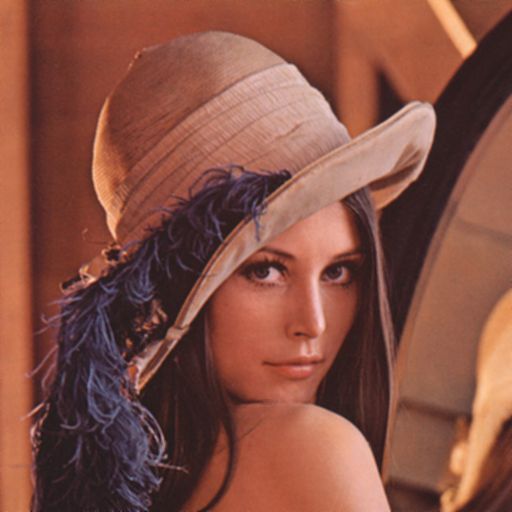
\includegraphics[width=\linewidth]{lenablurc.png}
  \caption{Blur C}
\endminipage\hfill
\minipage{0.2\textwidth}
  
\includegraphics[width=\linewidth]{lenablurdiffR.png}
  \caption{R channel}
\endminipage\hfill
\minipage{0.2\textwidth}
  
\includegraphics[width=\linewidth]{lenablurdiffG.png}
  \caption{G channel}
\endminipage\hfill
\minipage{0.2\textwidth}
  
\includegraphics[width=\linewidth]{lenablurdiffB.png}
  \caption{B channel}
\endminipage\hfill
\minipage{0.2\textwidth}%
  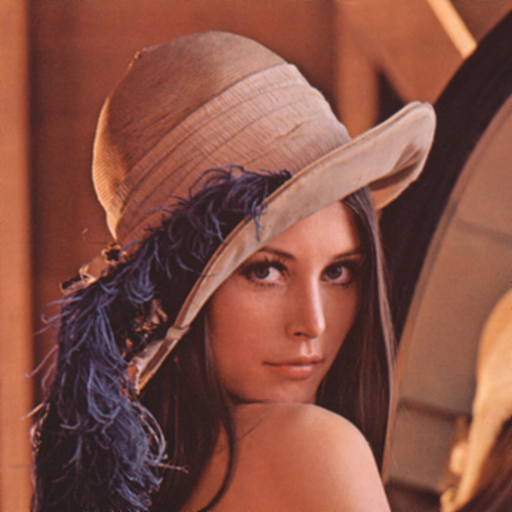
\includegraphics[width=\linewidth]{lenablurasm1.png}
  \caption{Blur ASM}
\endminipage
\end{figure}

Aunque las imágenes parecían exactamente iguales, habían diferencias en algunos píxeles. Estas diferencias se debían al redondeo hacia arriba llevado a cabo por la conversión desde float a entero. Mientras que el código en C redondeaba hacia abajo por defecto, las conversiones en ASM redondeaban hacia arriba por defecto.

Para resolver esto, existe un flag de SSE llamado $MXCSR$. Para mas información, ver la sección 10.2.3.1 del Volumen 1 de la guía de arquitectura Intel. Cada bit de este flag codifica algún comportamiento de las operaciones SSE. El valor por defecto de este flag es $0x1F80$. Para que redondee hacia abajo, utilizando la codificación de los bits del flag, había que poner el bit 12 y 13 en 1. Por lo tanto, simplemente setteamos el flag con la instrucción $ldmxcsr$ en $0x7F80$ y el algoritmo comenzó a andar sin problemas. Tuvimos esta misma problemática en todos los otros filtros más tarde.

\subsection{Experimentación}

Es fácil darse cuenta, ya sea mirando el código o comprendiendo qué es lo que debe hacer el algoritmo de Blur, de que todas las implementaciones del mismo van tener una complejidad temporal de $O(w*h)$, indicando que la cantidad de operaciones que realizará el algoritmo serán de orden cuadrático si tomamos $w = h = n$. Es decir, los gráficos que generemos deberán tener la forma de una parábola a medida que $n$ se vuelva más grande. Lo interesante, y he aquí donde radican las ventajas de hacer el código en Assembler, es que sabemos que las tres implementaciones diferirán en un múltiplo constante de las otras (por la definición de $O$). Intuitivamente, el código de ASM1 debería ir aproximadamente 3 veces más rápido por píxel que el de C, ya que procesa cada canal en paralelo con SIMD, y el código de ASM2 debería ser unas 4 veces más rápido que el de ASM1, ya que no sólo procesa los canales en paralelo, sino que además procesa los píxeles en grupos de a cuatro.

Cabe destacar, de cualquier forma, que nuestra intuición probablemente falle: tanto las optimizaciones que pueda llegar a realizar el compilador de C al código, así como también cuestiones de acceso a memoria en las distintas implementaciones (inclusive las instrucciones utilizadas en cada caso, o el branch predictor), y particularidades respecto del estado actual del sistema en el que se corren los experimentos pueden hacer variar los números obtenidos ampliamente, como veremos más adelante en el caso de HSL.

Haciendo un análisis poco delicado, observemos que la versión de ASM1 tiene 4 saltos condicionales, contra los 5 de ASM2, por lo que en principio, suponiendo que el branch predictor falle, la versión de ASM2 podría terminar siendo más cara. Por otro lado, el hecho de procesar de a 4 píxeles nos dará una ventaja difícil de estimar con respecto al ASM1. En términos del acceso a memoria, ambas versiones hacen uso de la memoria relativamente poco con respecto a los otros algoritmos, entrando solamente con fines de obtener las filas necesarias para procesar los datos, por lo que estimamos que en principio no debería ser el factor más importante, a pesar que todos los accesos que realizamos son desalineados.

Además, la performance de nuestros algoritmos de Blur no se verá afectada por ninguna otra característica de la imagen que el tamaño: ninguno de los algoritmos actúa según condiciones sobre el contenido de las imágenes. Las tres implementaciones simplemente procesan datos, sin comparar con ninguna otra cosa que no sea el número de columna o de fila. En concreto, esperamos que nuestras implementaciones en Assembler sean ambas más rápidas que la de C, y que entre ellas ASM2 sea más rápida que ASM1 (fundamentalmente por el procesamiento en paralelo de a muchos píxeles).

\begin{figure}[!b]
	\centering
  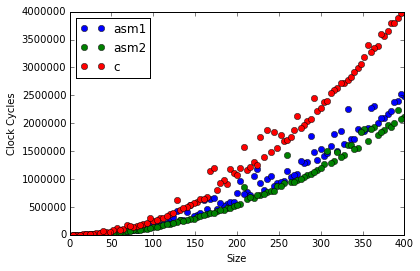
\includegraphics[width=10cm]{blur-imagenes-chicas.png}
  \caption{Performance de C compilado con -o3 y -ffastmath, ASM1 y ASM2. Utilizamos un conjunto de imágenes cuadrádas con tamaños múltiplos de 4 y píxeles tomados de una distribución uniforme, y medimos los resultados de 100 corridas, tomando como estadístico el mínimo de la cantidad de ciclos de reloj en todas las corridas.}
\end{figure}

Observemos que, efectivamente, se cumple lo que esperábamos: los ciclos de reloj crecen de forma cuadrática en relación al tamaño de la imagen. Además, notese que tienen relativamente poco desvío una implementación con respecto a la otra, suponemos que esto quiere decir que tienen comportamientos regulares con respecto al pipeline y sus accesos a memoria (de otra forma, tendríamos más picos en el gráfico). Nos sorprendió mucho que la implementación de ASM1 se asimile tanto a la de ASM2, ya que esperábamos una mayor amplitud entre las curvas; por esto, corrimos un nuevo experimento tomando tamaños de imagen mucho más grandes:

\begin{figure}[!hbt] 
	\centering
  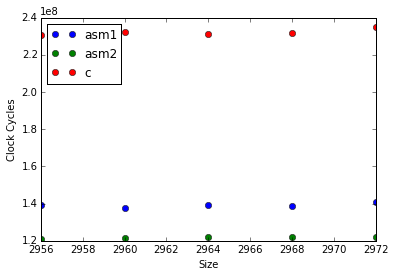
\includegraphics[width=10cm]{blur-imagenes-grandes.png}
  \caption{Performance de C compilado con -o3 y -ffastmath, ASM1 y ASM2. Utilizamos un conjunto de imágenes cuadradas con tamaños múltiplos de 4 y píxeles tomados de una distribución uniforme, y medimos los resultados de 100 corridas, tomando como estadístico el mínimo de la cantidad de ciclos de reloj en todas las corridas.}
\end{figure}

Esta vez, encontramos una brecha mucho más marcada entre las distintas implementaciones, lo que nos asegura que efectivamente el crecimiento de las constantes escondidas en la complejidad temporal está haciendo una diferencia importante a medida que aumenta la escala. Para finalizar, tomamos un ejemplo más de cerca para observar más precisamente las disparidades:

\begin{figure}[!hbt] 
	\centering
  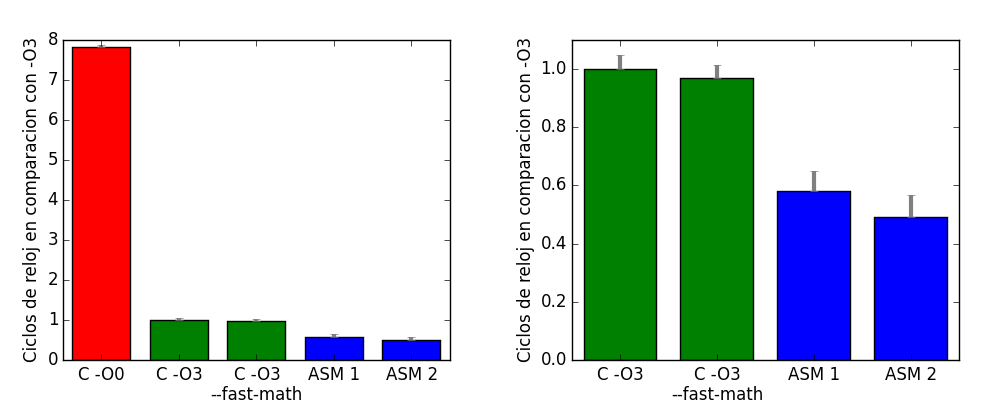
\includegraphics[width=17cm]{blur-all.png}
  \caption{Performance de C compilado con -o0, C compilado con -o3 y -ffastmath, ASM1 y ASM2. Utilizamos una imagen roja de $400 \times 400$, con píxeles tomados de una distribución uniforme, y medimos los resultados de 100 corridas, tomando como estadístico el mínimo de la cantidad de ciclos de reloj en todas las corridas.}
\end{figure}

Como habíamos notado antes, el hecho de estar utilizando imágenes pequeñas no ayuda a que se note la diferencia entre ASM1 y ASM2. Pensamos que uno de los posibles motivos para esto es que los algoritmos que escribimos no están optimizados en tanto a sus accesos a memoria: ambos hacen accesos desalineados. Una posible mejora para el algoritmo de ASM2 sería utilizar los registros AVX para poder obtener más píxeles de memoria, disminuyendo la cantidad de accesos, y permitiéndonos un trabajo mucho más rápido, procesando de a 8 píxeles en simultaneo. Otra posible mejora sería pedir que las direcciones de memoria con las que trabajamos estén alineadas a 16 bits. Esto nos permitiría realizar siempre accesos alineados, lo que debería mejorar la performance de nuestros algoritmos.

\newpage
\section{Experimentacion Blur}

\newpage

\section{Merge}

\subsection{C}
El código de C es bastante simple. Lo que hace al inicio es convertir ambos punteros a punteros a matrices de matrices, que tienen elementos de $w$ bytes de tamaño, que a su vez tienen elementos de 4 bytes de tamaño.

Luego se realizan 3 ciclos, el primero sobre las filas, el segundo sobre las columnas, y el tercero sobre los canales (exceptuando el canal de transparencia, notar que ii se inicializa en 1).

Finalmente se realiza la cuenta que se debe hacer para hacer el merge, convirtiendo todo adecuadamente (se convierte el valor del canal, que es un entero de 1 byte a float, se lo multiplica por value o 1-value según corresponda, se lo suma con el otro valor y se lo vuelve a convertir a entero de 8 bytes).

\subsection{ASM1}

En la primera versión del código de ASM, iniciamos guardando los parámetros que nos pasan en algunos registros auxiliares para no perderlos mas adelante.
Luego calculamos h*w dado que es la cantidad de iteraciones que vamos a realizar.

En el ciclo lo que hacemos es tener dos vectores de floats

\xmm{3}
\regfloats{$value$}{$value$}{$value$}{$1.0$}

\xmm{4}
\regfloats{$1-value$}{$1-value$}{$1-value$}{$0.0$}

Y levantamos de a un píxel, cuyos canales convertimos a float y multiplicamos por los registros exhibidos anteriormente. Luego convertimos a enteros de 8 bits nuevamente, empaquetando.

Notar que no se produce overflow. Tomemos por ejemplo el canal R, y supongamos que el valor del canal R para ambas imágenes es $255$.
Entonces $255value + 255(1-value)$ da $255$, que entra en 8 bits (si por errores de redondeo diera más, no importa, ya que el empaquetado lo hacemos saturado, entonces se queda en 255).

Finalmente escribimos en el lugar de la memoria correspondiente el valor obtenido y listo, repetimos este proceso hasta terminar.

Aunque en líneas generales esta rutina es igual a la de C, esperamos que tenga mejor rendimiento por dos razones.
Primero, en esta rutina tenemos que hacer menos saltos, dado que solo tenemos un ciclo, mientras que la versión de C tiene 2 ciclos.
Segundo, porque si el compilador no optimiza a la perfección las operaciones, es muy probable que realice las operaciones de los canales en serie, en vez de como lo hacemos nosotros, en paralelo.
Es decir, en el código de C los canales se van a procesar uno detrás del otro, mientras que en nuestro código se van a procesar todos juntos.


\subsection{ASM2}

Al igual que en la rutina anterior, luego de armar el stack frame guardamos los parámetros en algunos registros auxiliares para no perderlos. El resto del proceso es el mismo que antes, hasta que llegamos al precalculo de los vectores de $value$. Como aquí hay que hacer operaciones con enteros, en vez de punto flotante como antes, vamos a calcular las cosas de manera diferente.

En vez de guardarnos $value$, vamos a guardarnos $int16(256*value)$. ¿Por qué? Porque de esta manera vamos a poder cargar de a dos píxeles y hacer las operaciones mucho mas rápido que antes. Además así guardamos un valor que antes estaba entre 0 y 1 en un valor que esta entre 0 y 256, es decir, un valor que podemos representar con una buena aproximación entera.

De esta manera nos armamos el vector igual que antes, solo que multiplicado por 256. Luego lo pasamos a entero y luego lo empaquetamos consigo mismo en la parte alta.

De esta manera obtenemos en \xmm{3} los siguientes valores

\xmm{3}
\regintOcho{256$v$}{256$v$}{256$v$}{256}{256$v$}{256$v$}{256$v$}{256}

Donde $v$ es $value$.


Ahora, nos gustaría tener en el otro registros los números tal que, sumados con los de \xmm{3}, dan 256. Para eso, nos aprovechamos de la representación complemento a 2, dado que lo que queremos en realidad son los inversos aditivos (en 8 bits) de estos números en el registro \xmm{4}. Entonces usamos que el inverso aditivo de un número es el negado bit a bit más 1.

Cargamos en \xmm{4} 8 enteros de 16 bits con valor 257, ya que es 256+1.
Luego, al hacer la diferencia

\begin{lstlisting}
psubw xmm4, xmm3
\end{lstlisting}

obtenemos en \xmm{4} exactamente lo que queremos, es decir que si sumamos int16 a int16 en \xmm{3} y \xmm{4} da 256. Luego comenzamos el ciclo principal, que es muy similar al anterior.

Viendo esta implementación creemos que su desempeño va a ser aún mejor que el de la primera implementación en Assembler, dado que hacemos operaciones con números enteros que son mucho más rápidas que las operaciones con punto flotante. Sin embargo, hacer operaciones con números enteros implica un trade-off de velocidad por precisión, aunque el código es mucho mas rápido también es (muy poco) más inexacto. Analizaremos este error a continuación.

\subsubsection{Error}

En la segunda versión de merge se comete, obviamente, más error que en la primera, dado que estamos trabajando con enteros, debemos perder precisión cuando convertimos $256v$ a entero.

Por esta razón, aproximadamente el 30\% de las veces, el resultado difiere en más de 2 con el output de C de la cátedra. Esto se debe a que los métodos de cómputo son fundamentalmente distintos, uno con mucha mas precisión que la otra.

Pese a esto, el 100\% de los tests pasan con un error de 3, es decir, pese a que existe error, es despreciable. El error (por ejemplo, para el canal R) se puede expresar de la siguiente manera

$$\bigg|\lfloor R_1v\rfloor + \lfloor R_2(1-v) \rfloor
  -\bigg\lfloor \frac{R_1\lfloor 256v \rfloor}{256} \bigg\rfloor 
 -\bigg\lfloor \frac{R_2(256- \lfloor 256v) \rfloor)}{256} \bigg\rfloor\bigg| $$


$$\leq
\bigg|
\lfloor R_1v\rfloor - \bigg\lfloor \frac{R_1\lfloor 256v \rfloor}{256} \bigg\rfloor
\bigg|
+
\bigg|
\lfloor R_2(1-v) \rfloor -\bigg\lfloor \frac{R_2(256- \lfloor 256v) \rfloor)}{256} \bigg\rfloor
\bigg| $$

Se puede verificar fácilmente con Wolfram-Alpha o algún software similar que es es menor que 3.

\subsection{Experimentación}

Antes de comenzar a testear, supusimos que la performance de nuestros programas en Assembler iban a ser muy superiores a las de C. Creemos esto dado que vamos a aprovecharnos mejor de las utilidades de SSE que lo que puede hacer un compilador. 

Esperamos también que la performance mejore aún más en la segunda implementación, dado que todas las operaciones las realizamos con enteros en vez de con punto flotante.


\begin{figure}[!hbt] 
  \centering
  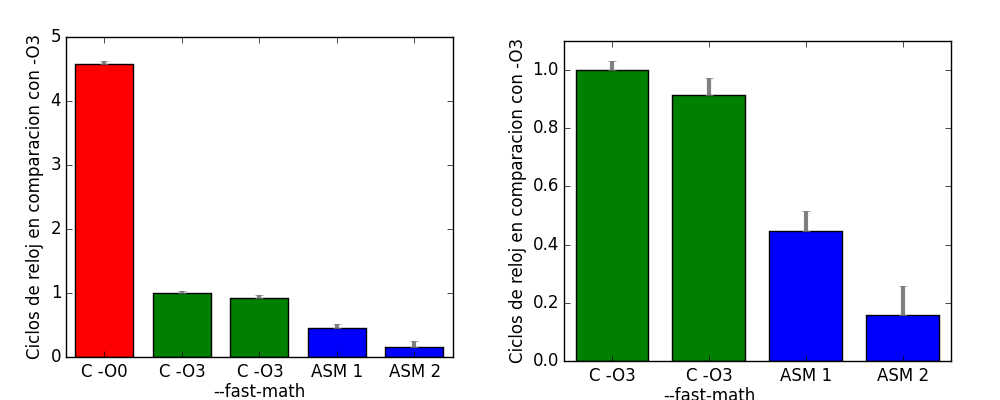
\includegraphics[scale=0.7]{merge-all.png}
  \caption{Comparación de la cantidad de ciclos de reloj utilizada por diferentes variantes de merge. Para tener una medida absoluta: la cantidad de ciclos de reloj promedio de C -O3 es 4,293,199. Tamaño de la muestra: 200 imagenes de $16 \times 10^4$ píxeles. Se indica el mínimo con la barra y el promedio con una linea gris.}
\end{figure}


Viendo los resultados, confirmamos nuestras hipótesis. De hecho, la performance de nuestros programas son mejores que las esperadas.

Como puede verse en los gráficos de escalabilidad, la performance de todos los algoritmos depende linealmente de la cantidad de píxeles de la imagen, sin embargo lo que cambia entre las diferentes implementaciones es la pendiente de esta función lineal.

La performance no depende de la imagen, dado que la operación que se realiza siempre es la misma, sin depender de los píxeles en cuestión.
Sin embargo, hay una cuestión con el error. Si el $\alpha$ que nos pasan por parámetro tiene muchos decimales detrás de la coma, es muy probable, y de hecho pasa, que nuestra segunda implementación en Assembler pierde precisión frente a la implementación de C. Esto fue explicado anteriormente, sin embargo creímos pertinente nombrarlo.

La única mejora que se nos ocurre para el código propuesto de Assembler es, si supiéramos que el inicio de la matriz está alineado a 16 bytes, entonces podríamos levantar de a 4 píxeles y analizarlos todos juntos (haciendo una especie de ciclo unrolling, es decir, teniendo 4 ciclos normales dentro de 1).
Esto es posible que mejore la performance, sin embargo es necesario como precondición que la matriz esté alineada a 16 bytes, ya que si no lo está y usamos una instrucción para leer alineado, los resultados serán desastrosos.

La comparación entre el programa de C y el de Assembler no es lo suficientemente justa. Esto se debe a que la versión de C por cada píxel, tiene 3 accesos a memoria, mientras que nuestra implementación tiene un acceso a memoria por píxel. Esto genera obviamente un speedup enorme, sobre todo en computadoras con memoria de velocidad limitada.
Aunque es posible que la gran mayoría de los accesos sean a cache, la performance ganada es significativa.

El acceso a memoria en nuestros códigos de Assembler es lo mínimo indispensable. La única mejora que se podría hacer con respecto al acceso a memoria es lo que fue nombrado anteriormente es la idea de hacer un unroll del ciclo y leer de a 4 píxeles, pero creemos que la performance no mejorará significativamente.

La diferencia entre operar con punto flotante y con enteros es significativa. Aunque ambas implementaciones en Assembler son mucho mas rápidas que la implementación de C, la que opera con enteros es nuevamente (bastante) más rápida que la que opera con punto flotante. Esto se debe a que en general las operaciones con enteros son mucho mas rápidas que las de punto flotante.

\newpage
\section{Experimentacion Merge}

\newpage

\section{HSL}

\subsection{C}
El código de C, al igual que el resto, es bastante sencillo. Lo que hace es loopear sobre todos los píxeles, hacer una conversión de RGB a HSL, hacer las sumas correspondientes, y luego volver a convertir a RGB.

Lo malo de la implementación es que el código sin optimizar de C hace más operaciones de las necesarias, ya que no usa todo el poder de las operaciones en SSE, que nosotros intentamos utilizar al máximo.

\subsection{ASM1}

En la versión primera versión del código de assembler la operatoriaes bastante distinta a la de C.
Al principio calculamos en xmm4 el vector de números que debemos sumarle a cada pixel hsl, con los parámetros que nos pasaron. De esta manera, 

\xmm{4}
\regfloats{l}{s}{h}{0}

Donde h,s,l son los que nos pasaron como parámetro y el 0 es lo que le tenemos que sumar a la transparencia (nada). Este registro tenemos que guardarlo en la pila, dado que cuando llamamos a rgbTOhsl, nos puede pisar los registros xmm pues la convención C no especifica nada sobre que no se puedan pisar (de hecho en algunos casos lo pisa, fue un bug que tardamos en encontrar).

También tenemos que malloc'ear un float para llamar a las funciones rgbTOhsl y hslTOrgb. Podríamos usar la pila, pero nos resultó mas fácil usar este método.

Luego comenzamos a loopear. 

Luego de convertir el pixel en cuestión de rgb a hsl, vamos a tener su valor en \xmm{3}.

\xmm{3}
\regfloats{LL}{SS}{HH}{AA}

Luego sumamos este registro con el registro que contiene los parámetros, como indica el filtro, de manera que queda

\xmm{3}
\regfloats{l+LL}{s+SS}{h+HH}{AA}

Va a ser útil para mas adelante tener un ejemplo, así que supongamos que \xmm{3} vale

\xmm{3}
\regfloats{0.5}{-0.322}{380}{255}


Ahora comienza la operatoria de saturación, entonces vamos a armar los siguientes registros

\xmm{5}
\regfloats{1-(l+LL)}{1-(s+SS)}{-360}{0}

\xmm{6}
\regfloats{-(l+LL)}{-(s+SS)}{360}{0}

Siguiendo el ejemplo anterior, los registros quedarían

\xmm{5}
\regfloats{0.5}{1.322}{-360}{0}

\xmm{6}
\regfloats{-0.5}{0.322}{360}{0}



Entonces procedemos a formar estos registros, usando la menor cantidad de instrucciones posibles, como siempre.

Luego nos armamos 2 registros más, que vamos a usar para las comparaciones

\xmm{12}
\regfloats{1}{1}{360}{256}

\xmm{13}
\regfloats{0}{0}{0}{0}


Luego comparamos estos registros con nuestro registro \xmm{3} (nótese que como SSE carece de comparaciones de mayor o igual, hay que dar vuelta los registros y hacer una comparacion de menor o igual).

Por lo tanto, con el ejemplo anterior, \xmm{12} y \xmm{13} quedan así:

\xmm{12}
\regfloats{0h}{0h}{ffffffffh}{0h}

\xmm{13}
\regfloats{0h}{ffffffffh}{0h}{0h}


Luego les hacemos un and entre los registros \xmm{12} y \xmm{5} y entre \xmm{13} y \xmm{6}, dword a dword, de manera seleccionar lo que vamos a querer sumar. En el ejemplo esto queda


\xmm{5}
\regfloats{0}{0}{-360}{0}

\xmm{6}
\regfloats{0}{0.322}{0}{0}

Recordemos el valor de \xmm{3}

\xmm{3}
\regfloats{0.5}{-0.322}{380}{255}


Ahora les sumamos estos registros a \xmm{3}, para terminar de llevar a cabo nuestro plan

\xmm{3}
\regfloats{0.5}{0}{320}{255}

Y listo, todo terminó como queríamos.

Ahora solo falta volver a convertir este numero a RGB y escribirlo a la memoria, de lo que se va a ocupar la funcion hslTOrgb.

\subsection{ASM2}

En la segunda implementación utilizamos fuertemente la primera.

Lo que hicimos en ambas rutinas de conversión es bastante directo, siguiendo los algoritmos proveidos por la cátedra. El mayor problema que tuvimos en ambas rutinas fue que tenemos que cargar constantemente constantes que vamos a usar durante los procesos. Esto hace que la ejecución de las rutinas de conversión sea mucho mas lenta de lo que podría ser si tuviéramos más registros para guardar las constantes que usamos todo el tiempo.

Este es definitivamente el factor más limitante de nuestra implementación y esperamos que impacte fuertemente en el rendimiento.



\newpage
\section{Experimentacion HSL}

\newpage
\section{Conclusiónes}

\end{document}
